\documentclass[tikz,border=15pt]{standalone}
\usepackage{tikz}
\usepackage{xcolor}
\usetikzlibrary{calc}

\definecolor{wallbg}{RGB}{250,240,230}
\definecolor{floorbg}{RGB}{156,99,56}
\definecolor{trimcolor}{RGB}{216,184,150}
\definecolor{plankcolor}{RGB}{125,78,42}
\definecolor{winblue}{RGB}{147,197,253}
\definecolor{gardengreen}{RGB}{74,222,128}
\definecolor{curtaincolor}{RGB}{254,215,170}
\definecolor{rodcolor}{RGB}{180,83,9}
\definecolor{picbg}{RGB}{254,243,199}
\definecolor{picsun}{RGB}{248,113,113}
\definecolor{pichill}{RGB}{52,211,153}
\definecolor{clockhand}{RGB}{30,41,59}
\definecolor{lamppole}{RGB}{120,53,15}
\definecolor{lampbase}{RGB}{69,26,3}
\definecolor{lampshade}{RGB}{253,224,71}
\definecolor{lampborder}{RGB}{234,179,8}
\definecolor{lampglow}{RGB}{254,240,138}
\definecolor{rugbg}{RGB}{254,243,199}
\definecolor{armback}{RGB}{154,52,18}
\definecolor{armbackborder}{RGB}{124,45,18}
\definecolor{armcushion}{RGB}{194,65,12}
\definecolor{armrest}{RGB}{234,88,12}
\definecolor{cardigan}{RGB}{77,124,15}
\definecolor{blanket}{RGB}{220,38,38}
\definecolor{slippers}{RGB}{236,72,153}
\definecolor{skincolor}{RGB}{254,215,170}
\definecolor{haircolor}{RGB}{203,213,225}
\definecolor{hairborder}{RGB}{148,163,184}
\definecolor{catmain}{RGB}{251,146,60}
\definecolor{catear}{RGB}{249,115,22}
\definecolor{tablewood}{RGB}{120,53,15}
\definecolor{tablecolor}{RGB}{146,64,14}
\definecolor{tabletop}{RGB}{180,83,9}
\definecolor{teapotcolor}{RGB}{6,95,70}
\definecolor{teacupbg}{RGB}{236,253,245}
\definecolor{teacupborder}{RGB}{167,243,208}
\definecolor{steamcolor}{RGB}{148,163,184}
\definecolor{tvbody}{RGB}{30,41,59}
\definecolor{tvscreen}{RGB}{125,211,252}
\definecolor{tvglow}{RGB}{56,189,248}
\definecolor{tvslot}{RGB}{41,37,36}
\definecolor{tvbase}{RGB}{51,65,85}
\definecolor{sunyellow}{RGB}{251,191,36}
\definecolor{hillgreen}{RGB}{34,197,94}
\definecolor{potcolor}{RGB}{234,88,12}
\definecolor{leafdark}{RGB}{21,128,61}
\definecolor{leafmid}{RGB}{22,163,74}
\definecolor{leafbright}{RGB}{34,197,94}

\begin{document}
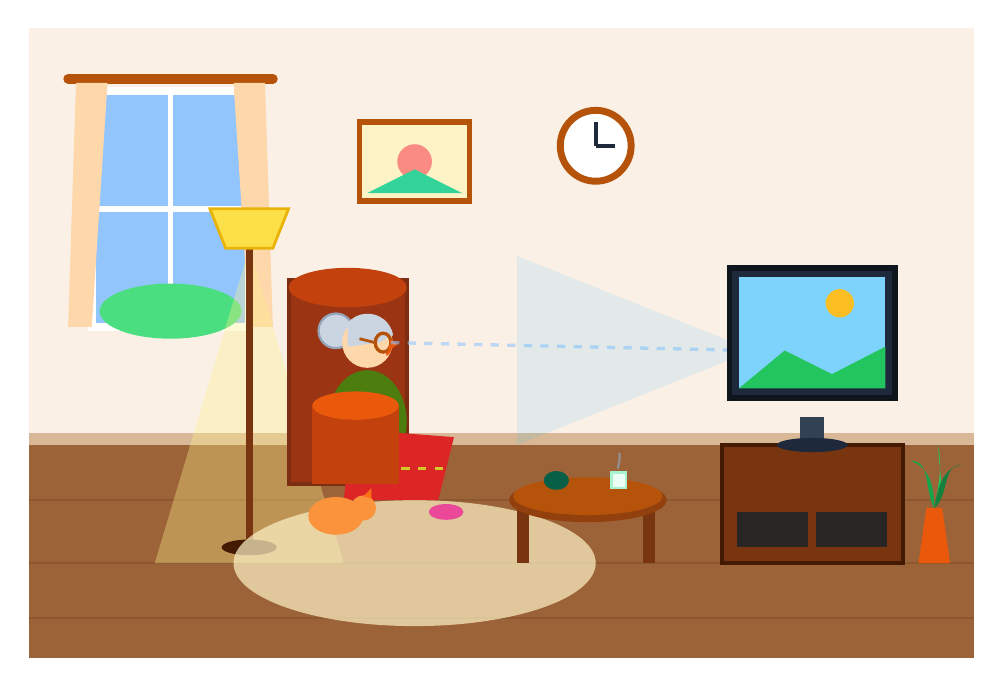
\begin{tikzpicture}

% 1. ROOM WALL & FLOOR
\fill[wallbg] (-6,-4) rectangle (6,4);
\fill[floorbg] (-6,-4) rectangle (6,-1.2);
\fill[trimcolor] (-6,-1.3) rectangle (6,-1.15);
\draw[plankcolor, opacity=0.5, line width=0.8pt] (-6,-2.0) -- (6,-2.0);
\draw[plankcolor, opacity=0.5, line width=0.8pt] (-6,-2.8) -- (6,-2.8);
\draw[plankcolor, opacity=0.5, line width=0.8pt] (-6,-3.5) -- (6,-3.5);

% 2. WINDOW (Left)
\fill[winblue] (-5.2, 0.2) rectangle (-3.2, 3.2);
\draw[white, line width=3pt] (-5.2, 0.2) rectangle (-3.2, 3.2);
\draw[white, line width=2pt] (-4.2, 0.2) -- (-4.2, 3.2);
\draw[white, line width=2pt] (-5.2, 1.7) -- (-3.2, 1.7);
\fill[gardengreen] (-4.2, 0.4) ellipse (0.9cm and 0.35cm);
% Curtain & Rod
\draw[rodcolor, line width=3.5pt, line cap=round] (-5.5, 3.35) -- (-2.9, 3.35);
\fill[curtaincolor] (-5.4, 3.3) -- (-5.0, 3.3) -- (-5.2, 0.2) -- (-5.5, 0.2) -- cycle;
\fill[curtaincolor] (-3.4, 3.3) -- (-3.0, 3.3) -- (-2.9, 0.2) -- (-3.2, 0.2) -- cycle;

% Wall Picture Frame
\draw[draw=rodcolor, fill=picbg, line width=2pt] (-1.8, 1.8) rectangle (-0.4, 2.8);
\fill[picsun, opacity=0.8] (-1.1, 2.3) circle (0.22cm);
\fill[pichill] (-1.7, 1.9) -- (-1.1, 2.2) -- (-0.5, 1.9) -- cycle;

% Wall Clock
\fill[white, draw=rodcolor, line width=2.5pt] (1.2, 2.5) circle (0.45cm);
\draw[clockhand, line width=1.5pt] (1.2, 2.5) -- (1.2, 2.8);
\draw[clockhand, line width=1.5pt] (1.2, 2.5) -- (1.45, 2.5);

% 3. FLOOR LAMP
\fill[lampglow, opacity=0.35] (-3.2, 1.2) -- (-4.4, -2.8) -- (-2.0, -2.8) -- cycle;
\draw[lamppole, line width=2.5pt] (-3.2, -2.6) -- (-3.2, 1.5);
\fill[lampbase] (-3.2, -2.6) ellipse (0.35cm and 0.1cm);
\fill[lampshade, draw=lampborder, line width=1pt] (-3.5, 1.2) -- (-2.9, 1.2) -- (-2.7, 1.7) -- (-3.7, 1.7) -- cycle;

% 4. COZY RUG
\fill[rugbg, opacity=0.7] (-1.1, -2.8) ellipse (2.3cm and 0.8cm);

% 5. GRANDMOTHER IN ARMCHAIR
% Armchair backrest
\fill[armback, draw=armbackborder, line width=1.5pt] (-2.7, -1.8) rectangle (-1.2, 0.8);
\fill[armcushion] (-1.95, 0.7) ellipse (0.75cm and 0.25cm);

% Grandma Body (Green cardigan)
\fill[cardigan] (-1.7, -1.0) ellipse (0.5cm and 0.65cm);

% Blanket on lap
\fill[blanket] (-2.0, -2.0) -- (-0.8, -2.0) -- (-0.6, -1.2) -- (-1.9, -1.1) -- cycle;
\draw[yellow!80!black, dashed, line width=1.2pt] (-1.9, -1.6) -- (-0.7, -1.6);

% Slippers
\fill[slippers] (-0.7, -2.15) ellipse (0.22cm and 0.1cm);

% Grandma Head (Profile looking right towards TV)
\fill[haircolor, draw=hairborder, line width=0.8pt] (-2.1, 0.15) circle (0.22cm);
\fill[skincolor] (-1.7, 0.0) circle (0.32cm);
\fill[haircolor] (-1.95, 0.25) arc (140:10:0.33) -- (-1.55, 0.0) -- (-1.95, -0.05) -- cycle;
% Glasses & Smile
\draw[draw=rodcolor, line width=1.2pt] (-1.5, 0.0) ellipse (0.1cm and 0.12cm);
\draw[draw=rodcolor, line width=1.0pt] (-1.6, 0.0) -- (-1.8, 0.05);
\draw[draw=armrest, line width=1.2pt, line cap=round] (-1.4, 0.02) -- (-1.35, -0.02) -- (-1.4, -0.06);
\draw[draw=armrest, line width=1.0pt, line cap=round] (-1.45, -0.15) arc (-50:10:0.12);

% Armrest
\fill[armcushion] (-2.4, -1.8) rectangle (-1.3, -0.8);
\fill[armrest] (-1.85, -0.8) ellipse (0.55cm and 0.18cm);

% Sleeping Cat
\fill[catmain] (-2.1, -2.2) ellipse (0.35cm and 0.24cm);
\fill[catmain] (-1.75, -2.1) circle (0.16cm);
\fill[catear] (-1.75, -1.95) -- (-1.65, -1.85) -- (-1.65, -1.98) -- cycle;

% 6. TEA TABLE
\fill[tablewood] (0.2, -2.8) rectangle (0.35, -2.0);
\fill[tablewood] (1.8, -2.8) rectangle (1.95, -2.0);
\fill[tablecolor] (1.1, -2.0) ellipse (1.0cm and 0.28cm);
\fill[tabletop] (1.1, -1.95) ellipse (0.95cm and 0.24cm);

% Teapot & Cup
\fill[teapotcolor] (0.7, -1.75) ellipse (0.16cm and 0.12cm);
\fill[teacupbg, draw=teacupborder, line width=0.8pt] (1.4, -1.85) rectangle (1.58, -1.65);
\draw[steamcolor, opacity=0.7, line width=0.8pt] (1.48, -1.6) to[out=80, in=-80] (1.5, -1.4);

% 7. TV & STAND (Right)
% Line of sight (dotted blue arrow from grandma to TV)
\draw[winblue, line width=1.2pt, dashed, opacity=0.6] (-1.4, 0.0) -- (3.2, -0.1);

% TV Light Cone
\fill[tvglow, opacity=0.12] (3.2, -0.1) -- (0.2, 1.1) -- (0.2, -1.3) -- cycle;

% TV Cabinet
\fill[tablewood, draw=lampbase, line width=1.5pt] (2.8, -2.8) rectangle (5.1, -1.3);
\fill[tvslot] (3.0, -2.6) rectangle (3.9, -2.15);
\fill[tvslot] (4.0, -2.6) rectangle (4.9, -2.15);

% TV Stand Base
\fill[tvbase] (3.8, -1.3) rectangle (4.1, -0.95);
\fill[tvbody] (3.95, -1.3) ellipse (0.45cm and 0.09cm);

% TV Monitor & Screen
\fill[tvbody, draw=tvbody!50!black, line width=2pt] (2.9, -0.7) rectangle (5.0, 0.95);
\fill[tvscreen] (3.02, -0.58) rectangle (4.88, 0.83);
% Landscape broadcast on TV
\fill[sunyellow] (4.3, 0.5) circle (0.18cm);
\fill[hillgreen] (3.02, -0.58) -- (3.6, -0.1) -- (4.2, -0.4) -- (4.88, -0.05) -- (4.88, -0.58) -- cycle;

% Houseplant (Far Right)
\fill[potcolor] (5.3, -2.8) -- (5.7, -2.8) -- (5.6, -2.1) -- (5.4, -2.1) -- cycle;
\fill[leafmid] (5.5, -2.1) to[out=120, in=0] (5.2, -1.5) to[out=-20, in=90] (5.5, -2.1);
\fill[leafbright] (5.5, -2.1) to[out=80, in=-80] (5.55, -1.3) to[out=-90, in=60] (5.5, -2.1);
\fill[leafdark] (5.5, -2.1) to[out=40, in=180] (5.85, -1.55) to[out=190, in=80] (5.5, -2.1);

\end{tikzpicture}
\end{document}
